%e) Bootstrap
\documentclass{article}
\usepackage{tikz}
\definecolor{mycolor}{HTML}{DAE8FC}
\definecolor{mycolor2}{HTML}{EDDAFC}
\definecolor{mycolor3}{HTML}{FFBE97}
\begin{document}

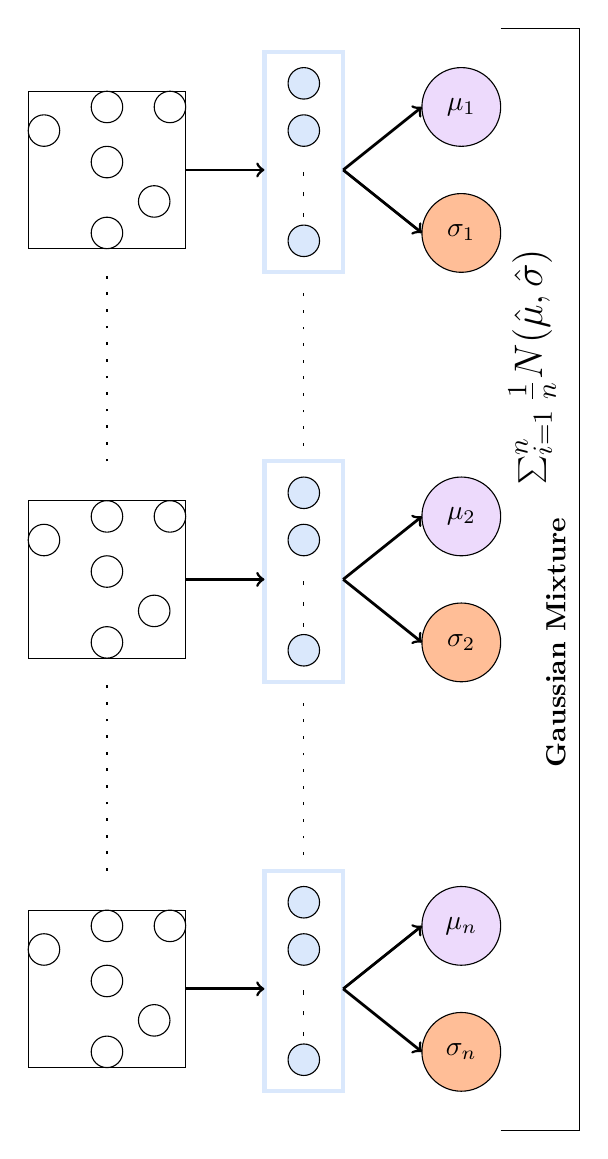
\begin{tikzpicture}

% Model 1
    % Rectangle
    \draw[color=mycolor, line width = 1.5pt] (0, 5.9) rectangle (1, 8.7);
    
    % Nodes in the hidden layer
    \foreach \i in {1,2} {
        \draw[fill=mycolor] (0.5, \i*0.6 + 7.1) circle (0.2cm); 
    }
    \draw[fill=mycolor] (0.5, 6.3) circle (0.2cm);

    % Dashes in rectangle between nodes
    \draw[dotted, dash pattern=on 1.5pt off 6.0pt] (0.5, 6.6) -- (0.5, 7.2);

    % Output nodes for Model 1
    % Mean1
    \draw[fill=mycolor2] (2.5, 8) circle (0.5cm);
    \node at (2.5, 8) {$ \mu_{1}$};
    % Sigma1
    \draw[fill=mycolor3] (2.5, 6.4) circle (0.5cm);
    \node at (2.5, 6.4) {$\sigma_{1}$};
    
% Model 2
    % Rectangle
    \draw[color=mycolor, line width = 1.5pt] (0, 0.7) rectangle (1, 3.5);    
    % Nodes in the hidden layer
    \foreach \i in {1,2} {
        \draw[fill=mycolor] (0.5, \i*0.6 + 1.9) circle (0.2cm); 
    }
    \draw[fill=mycolor] (0.5, 1.1) circle (0.2cm);

    % Dashes in rectangle between nodes
    \draw[dotted, dash pattern=on 1.5pt off 6.0pt] (0.5, 1.4) -- (0.5, 2.0); 

    % Output nodes for Model 2
    % Mean2
    \draw[fill=mycolor2] (2.5, 2.8) circle (0.5cm);
    \node at (2.5, 2.8) {$ \mu_{2}$};  
    % Sigma2
    \draw[fill=mycolor3] (2.5, 1.2) circle (0.5cm);
    \node at (2.5, 1.2) {$\sigma_{2}$};

% Model N
    % Rectangle
    \draw[color=mycolor, line width = 1.5pt] (0, -4.5) rectangle (1, -1.7); 

    % Nodes in the hidden layer
    \foreach \i in {1,2} {
        \draw[fill=mycolor] (0.5, \i*0.6 + -3.3) circle (0.2cm); 
    }
    
    % Dashes in rectangle between nodes
    \draw[fill=mycolor] (0.5, -4.1) circle (0.2cm);
    \draw[dotted, dash pattern=on 1.5pt off 6.0pt] (0.5, -3.8) -- (0.5, -3.2); 

    % Output nodes for Model N
    % MeanN
    \draw[fill=mycolor2] (2.5, -2.4) circle (0.5cm);
    \node at (2.5, -2.4) {$ \mu_{n}$}; 
    % SigmaN
    \draw[fill=mycolor3] (2.5, -4) circle (0.5cm);
    \node at (2.5, -4) {$\sigma_{n}$};

    %Between Dotted lines:
    \draw[dotted, dash pattern=on 1.0pt off 5.0pt] (0.5, -1.5) -- (0.5, 0.5);
    
    \draw[dotted, dash pattern=on 1.0pt off 5.0pt] (0.5, 3.7) -- (0.5, 5.7);

    %Between Squares, Dotted lines:
    \draw[dotted, dash pattern=on 1.0pt off 5.0pt] (-2, -1.7) -- (-2, 0.7);
    
    \draw[dotted, dash pattern=on 1.0pt off 5.0pt] (-2, 3.5) -- (-2, 5.9);
    
% Datasets
    %Dataset1
    % Square
    \draw (-3, 6.2) rectangle (-1, 8.2);
    % Datapoints
    \draw (-2, 6.4) circle (0.2cm);
    \draw (-2, 7.3) circle (0.2cm);
    \draw (-2, 8) circle (0.2cm);
    \draw (-1.2, 8) circle (0.2cm);
    \draw (-2.8,7.7) circle (0.2cm);
    \draw (-1.4, 6.8) circle (0.2cm);

    %Dataset2
    % Square
    \draw (-3, 1) rectangle (-1, 3);
    % Datapoints
    \draw (-2, 1.2) circle (0.2cm);
    \draw (-2, 2.1) circle (0.2cm);
    \draw (-2, 2.8) circle (0.2cm);
    \draw (-1.2, 2.8) circle (0.2cm);
    \draw (-2.8, 2.5) circle (0.2cm);
    \draw (-1.4, 1.6) circle (0.2cm);

    %DatasetN
    % Square
    \draw (-3, -4.2) rectangle (-1, -2.2);
    % Datapoints
    \draw (-2, -4) circle (0.2cm);
    \draw (-2, -3.1) circle (0.2cm);
    \draw (-2, -2.4) circle (0.2cm);
    \draw (-1.2, -2.4) circle (0.2cm);
    \draw (-2.8, -2.7) circle (0.2cm);
    \draw (-1.4, -3.6) circle (0.2cm);
       
    % Arrows connecting data to hidden layers and output node
    \draw[->,  line width=1pt] (-1, 2) -- (0, 2);
    \draw[->,  line width=1pt] (-1, 7.2) -- (0, 7.2);
    \draw[->,  line width=1pt] (-1, -3.2) -- (0, -3.2);
    
    % Model2 arrows
    \draw[->,  line width=1pt] (1, 2) -- (2, 2.8);
    \draw[->,  line width=1pt] (1, 2) -- (2, 1.2);
    % Model1 arrows
    \draw[->,  line width=1pt] (1, 7.2) -- (2, 8);
    \draw[->,  line width=1pt] (1, 7.2) -- (2, 6.4);
    % ModelN arrows
    \draw[->,  line width=1pt] (1, -3.2) -- (2, -2.4);
    \draw[->,  line width=1pt] (1, -3.2) -- (2, -4);

    %right side lines
    \draw (4,-5) -- (4,9);
    \draw (3,9) -- (4,9);
    \draw (3,-5) -- (4,-5);

    % Right text
    \node[rotate=90, font=\bfseries] at (3.7, 1.2) {Gaussian Mixture};
    \node[rotate=90,font=\fontsize{14}{18}\selectfont\bfseries] at (3.4, 4.7) 
    {$\sum_{i=1}^{n}\frac{1}{n}N(\hat{\mu}, \hat{\sigma})$};

    
\end{tikzpicture}
\end{document}